\documentclass[aspectratio=169]{beamer}

%%% Работа с русским языком
\usepackage{cmap}					% поиск в PDF
\usepackage{mathtext} 				% русские буквы в формулах
\usepackage[T2A]{fontenc}			% кодировка
\usepackage[utf8]{inputenc}			% кодировка исходного текста
\usepackage[english,russian]{babel}	% локализация и переносы
\usepackage{indentfirst}
\frenchspacing

%%% Дополнительная работа с математикой
\usepackage{amsmath,amsfonts,amssymb,amsthm,mathtools}  % AMS

%%% Текст в колонки
\usepackage{multicol}

%%% Системы уравнений
\usepackage{cases}

%%% Таблицы
\usepackage{array}

%%% Картинки
\usepackage{graphicx}
\usepackage{float}

%%% Список литературы
\usepackage[sorting=none]{biblatex}
\renewbibmacro{in:}{\ifentrytype{article}
    {}
    {\bibstring{in}\printunit{\intitlepunct}}
}
\addbibresource{references.bib}

%%% Гиперссылки
\usepackage{hyperref}

%%% Перенос знаков в формулах (по Львовскому)
\newcommand*{\hm}[1]{#1\nobreak\discretionary{}
{\hbox{$\mathsurround=0pt #1$}}{}}


%%% Свои команды

\newcommand*{\No}{\textnumero}

\newcommand{\vect}[1]{\textbf{\textit{#1}}}
\newcommand{\vx}{{\vect{x}}}

\newcommand{\avphi}{{\widetilde{\phi}}}

\newcommand{\half}{\cfrac{1}{2}}

\newcommand{\partt}[1]{\cfrac{\partial #1}{\partial t}}
\newcommand{\partx}[1]{\cfrac{\partial #1}{\partial x}}
\newcommand{\partxx}[1]{\cfrac{\partial^2 #1}{\partial x^2}}
\newcommand{\partr}[1]{\cfrac{\partial #1}{\partial r}}

\newcommand{\gradscalsq}[1]{\left( \nabla #1, \nabla #1 \right)}

\newcommand{\Natural}{{\mathbb{N}}}
\newcommand{\Real}{{\mathbb{R}}}
\newcommand{\bigO}{{\mathcal{O}}}
\newcommand{\clOmega}{{\overline{\Omega}}}

\newcommand{\norm}[1]{\| #1 \|}
\newcommand{\enorm}{{\| \cdot \|}}

\newcommand{\plapl}[2]{\Div(\norm{\nabla #1}_2^{#2} \nabla #1)}
\newcommand{\bilapl}[1]{\Delta^2 #1}

\newcommand{\gridfunc}[1]{\left[ #1 \right]}


%%% Свои операторы
\DeclareMathOperator{\Div}{{div}}
\DeclareMathOperator{\Const}{{const}}

%%% Цвета
\definecolor{green}{RGB}{0,200,0}
\definecolor{red}{RGB}{200,0,0}

%%% Тема оформления
\usetheme{Madrid}


%%% Титульный лист
\title[Электрический пробой]{Моделирование канала электрического пробоя \\ методом диффузной границы}
\author[]{
	\underline{Пономарев А. С.}\textsuperscript{1,2}, Савенков Е. Б.\textsuperscript{2}, Зипунова Е. В.\textsuperscript{2}
}
\institute[]{
	\textsuperscript{1}МФТИ (НИУ) \\
	\textsuperscript{2}ИПМ им. М. В. Келдыша РАН
}
\date[]{
	Вычислительная классическая и многофазная \\ гидродинамика и термомеханика сплошной среды \\
	\vspace{3mm}
	4--8 ноября 2024 года
}
\logo{
\includegraphics[height=0.8cm]{../figures/labels.jpg}}


\begin{document}

\AtBeginSection[]{
	\begin{frame}{Содержание}
	\Large
	\tableofcontents[currentsection]
	\end{frame}
}

\begin{frame}
\titlepage
\end{frame}

\begin{frame}{Содержание}
\Large
\tableofcontents
\end{frame}

%!TEX root = ../main.tex

\section{Введение}

Электрический пробой~-- это явление резкого возрастания тока в диэлектрике при приложении электрического напряжения выше некоторого критического значения. Механизм разрушения диэлектрика под действием электрического поля сложен и многообразен: оно может иметь различные причины, характер развития, сопутствующие физические процессы \cite{vorobiev_dielectric_physics}.

Среди многообразия математических моделей, созданных для описания развития канала электрического пробоя, выделим предложенную в работе \cite{pitike_dielectric_breakdown} модель типа диффузной границы.

В настоящее время модели типа диффузной границы составляют целый класс подходов для решения задач в различных областях науки и техники. В частности, описанная в работе \cite{pitike_dielectric_breakdown} модель построена как формальное обобщение ранее известных моделей типа диффузной границы, применяемых в теории трещин.

Исследование и дальнейшее развитие упомянутой модели можно найти в работах \cite{zipunova_higher_codimension, zipunova_conservative, zipunova_thermomechanical, ponomarev_stability}. Основные положения метода диффузной границы в применении к моделированию развития канала электрического пробоя перечислены в работе \cite{ponomarev_stability}.

Модели типа диффузной границы используются для описания систем, в которых вещество может находиться в нескольких различных состояниях~-- фазах,~-- причем вещество в одной и той же фазе образует некоторые однородные области. В моделях типа диффузной границы распределение фаз вещества задается гладкой функцией $\phi$~-- фазовым полем,~-- которая в каждой области однородности близка к постоянной. Характерная толщина разделяющего слоя (<<диффузной границы>>) и, соответственно, скорость изменения~$\phi$ при переходе от одной фазы к другой определяется параметрами модели.

В работе \cite{zipunova_higher_codimension} проводится исследование свойства упомянутой модели развития канала электрического пробоя, которое можно назвать коразмерностью <<включений>>. Для задач теории трещин естественным будет двумерное включение (плоская трещина) в трехмерной среде вещества~-- в таком случае говорят, что коразмерность объекта равна 1. Обратим внимание, что, хотя исследуемая модель, как было сказано, получена на основе моделей из теории трещин, для нее характерным будет одномерное включение (канал пробоя), то есть имеющее коразмерность 2. В работе \cite{zipunova_higher_codimension} указано, что это может привести к нетривиальным последствиям, и предложено определенное обобщение исходной модели, которое предположительно делает ее более адекватной.

Суть обобщения состоит в формальном добавлении в уравнения модели двух слагаемых высших порядков с некоторыми коэффициентами. Целью настоящей работы является численная проверка поведения модели при различных значениях коэффициентов. Для этого ищется стационарное распределение фазового поля $\phi$ в нескольких характеристических случаях. Построение разностной схемы для задачи несет определенные сложности, связанные с необходимостью задать граничные условия на множествах коразмерности~2 и~3 в трехмерном пространстве. Предполагается, что точках этих множеств функция фазового поля $\phi$ имеет особенность.

Авторами применена модификация метода конечных объемов. Для части конфигураций обобщенной модели она позволила составить разнотную схему. Создана компьютерная программа, реализующая схему; проделаны расчеты, их результаты приведены в виде графиков. Для остальных конфигураций модели в процессе применения метода возникли фундаментальные проблемы, что позволяет выдвинуть гипотезу о некорректной постановке дифференциальной задачи в этих случаях.

%!TEX root = ../main.tex

\section{Постановка задачи}

\begin{frame}{Одномерная задача}
\vspace{-0.3cm}
\begin{itemize}
	\item Область $\clOmega = [0, W]_x \times [0, H]_y \times I_z$ в форме параллелепипеда
	\item $\phi(\vx, 0) = \phi_0(\vx) = \phi_0(x)$, $\epsilon_0(\vx) = \epsilon_0(x)$ не зависят от $y$ и $z$
	\item $\Phi|_{y = 0} = \Phi^- \in \mathbb{R}$, $\Phi|_{y = h} = \Phi^+ \in \mathbb{R}$
\end{itemize}
Подробнее в работе \cite{ponomarev_stability}. \\[0.3cm]
Решением является функция электрического потенциала
\begin{columns}
\column{0.65\textwidth}
	\vspace{-1cm}
	$$\Phi(\vx, t) = \Phi^- \hm + \cfrac{y}{h}(\Phi^+ - \Phi^-).$$
\column{0.35\textwidth}
	\begin{figure}
		\vspace*{-2.3cm}
		\hspace*{0.5cm}
		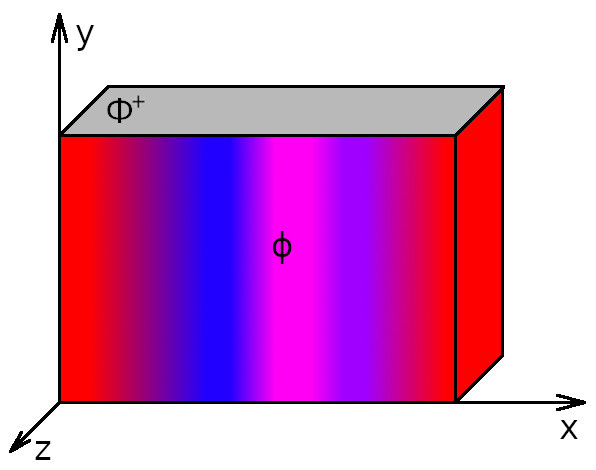
\includegraphics[width=0.85\textwidth]{figures/one_dim_problem.jpg}
	\end{figure}
\end{columns}
\vspace{-0.4cm}
Тогда уравнение на $\phi$ принимает вид
\begin{block}{}
	$$\cfrac{1}{m} \partt{\phi} = \half K_\Phi^2 \epsilon'(\phi) + \cfrac{\Gamma}{l^2} f'(\phi) + \half \Gamma \partxx{\phi}$$
\end{block}
$K_\Phi = \cfrac{\Phi^+ - \Phi^-}{h} = \norm{\nabla \Phi}$. Будем считать $\epsilon_0 = \Const$.
\end{frame}


\section{Теоретический анализ}

\begin{frame}{Анализ положений равновесия}
\begin{itemize}
	\item Канал пробоя может развиваться из малых возмущений свойств неповрежденной среды. Выясним условия развития.
	\item Рассмотрим положения равновесия вида $\phi(x, t) \equiv C$. Положению равновесия соответствует ноль $C$ функции
\end{itemize}
$$\chi(\phi) = \half K_\Phi^2 \epsilon'(\phi) + \cfrac{\Gamma}{l^2} f'(\phi).$$
\vspace{-0.5cm}
\begin{itemize}
	\item Исследуем положения равновесия на устойчивость спектральным методом: к $\phi \equiv C$ прибавим возмущение $\delta \phi = e^{\alpha t} \cos(\omega x)$, линеаризуем уравнение на $\delta \phi$.
	\item $\chi(\phi)$ возрастает в $C \Longrightarrow$ равновесие неустойчиво; $\chi(\phi)$ убывает в $C \Longrightarrow$ равновесие устойчиво.
\end{itemize}
\end{frame}


\begin{frame}{Анализ положений равновесия}
\vspace{-0.9cm}
\begin{columns}
\column{0.3\textwidth}
	\begin{center}
		<<Слабое>> напряжение
	\end{center}
	\vspace{-0.2cm}
	$$0 \leqslant \cfrac{K_\Phi^2 l^2 \epsilon_0}{2 \Gamma} < \delta^2$$
	\vspace{-0.7cm}
	\begin{figure}
		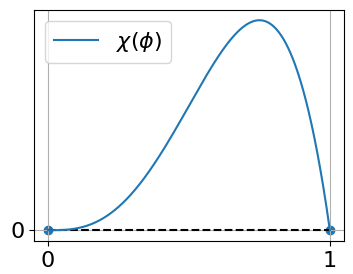
\includegraphics[width=\textwidth]{figures/equilibriums_case_1.png}
	\end{figure}
\column{0.3\textwidth}
	\begin{center}
		<<Среднее>> напряжение
	\end{center}
	\vspace{-0.2cm}
	$$\delta^2 < \cfrac{K_\Phi^2 l^2 \epsilon_0}{2 \Gamma} < (1 + \delta)^2$$
	\vspace{-0.7cm}
	\begin{figure}
		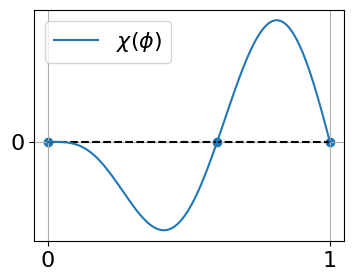
\includegraphics[width=\textwidth]{figures/equilibriums_case_2.png}
	\end{figure}
\column{0.3\textwidth}
	\begin{center}
		<<Сильное>> напряжение
	\end{center}
	\vspace{-0.2cm}
	$$(1 + \delta)^2 < \cfrac{K_\Phi^2 l^2 \epsilon_0}{2 \Gamma}$$
	\vspace{-0.7cm}
	\begin{figure}
		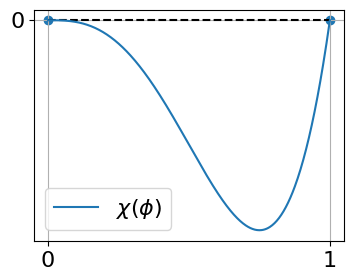
\includegraphics[width=\textwidth]{figures/equilibriums_case_3.png}
	\end{figure}
\end{columns}
\begin{columns}
\column{0.3\textwidth}
	\hspace{0.5cm}
	$\phi \equiv 0$ неустойчивое \\
	\hspace{0.5cm}
	$\phi \equiv 1$ устойчивое
\column{0.3\textwidth}
	\hspace{0.5cm}
	$\phi \equiv 0$ устойчивое \\
	\hspace{0.5cm}
	$\phi \equiv С_3$ неустойчивое \\
	\hspace{0.5cm}
	$\phi \equiv 1$ устойчивое
\column{0.3\textwidth}
	\hspace{0.5cm}
	$\phi \equiv 0$ устойчивое \\
	\hspace{0.5cm}
	$\phi \equiv 1$ неустойчивое
\end{columns}
\end{frame}


\section{Численный анализ}

\begin{frame}{Разностная схема}
\begin{block}{Разностная задача}
	$$\cfrac{1}{m} \cfrac{\phi_i^{j + 1} - \phi_i^j}{\tau} = \half K_\phi^2 \epsilon'(\phi_i^j) + \cfrac{\Gamma}{l^2} f'(\phi_i^j) + \cfrac{\Gamma}{2} \cfrac{\phi_{i + 1}^j - 2 \phi_i^j + \phi_{i - 1}^j}{h^2}$$
	$$\phi_i^0 = \phi_0(ih); \quad \phi_0^j = \phi_l(j \tau); \quad \phi_n^j = \phi_r(j \tau)$$
	Сетка регулярная; $\tau$ -- шаг по времени, $h$ -- шаг по пространству.
\end{block}
Явная разностная схема первого порядка по времени, второго -- по пространству.
\end{frame}


\begin{frame}{Оценка устойчивости}
\begin{itemize}
	\item Рассмотрим возмущенное решение $\phi_i^j + \delta_i^j$. Линеаризуем уравнение на возмущение $\delta_i^j$ в точке $\phi_i^j = P$:
\end{itemize}
$$\delta_i^{j + 1} = \delta_i^j + m \tau \left( \half K_\Phi^2 \epsilon''(P) \delta_i^j + \cfrac{\Gamma}{l^2} f''(P) \delta_i^j + \cfrac{\Gamma}{2} \cfrac{\delta_{i + 1}^j - 2 \delta_i^j + \delta_{i - 1}^j}{h^2} \right).$$
\begin{itemize}
	\item Применим спектральный признак устойчивости:
\end{itemize}
$$1 > | \lambda(\theta) | = \left| 1 + m \tau \left( \half K_\Phi^2 \epsilon''(P) + \cfrac{\Gamma}{l^2} f''(P) - \cfrac{2 \Gamma}{h^2} \sin^2 \cfrac{\theta}{2} \right) \right|.$$
\begin{itemize}
	\item Исследуем вблизи $P = 0$.
\end{itemize}
\end{frame}


\begin{frame}{Оценка устойчивости}
\begin{block}{Условие устойчивости}
	$$\tau \leqslant \cfrac{1}{2 m} \left( \cfrac{K_\Phi^2 \epsilon_0}{\delta^{5/3}} + \cfrac{\Gamma}{h^2} \right)^{-1}$$
\end{block}
\begin{block}{Упрощенное условие устойчивости}
	$$\tau \leqslant \cfrac{1}{4 m} \min \left(\cfrac{\delta^{5/3}}{K_\Phi^2 \epsilon_0}, \; \cfrac{h^2}{\Gamma} \right)$$
\end{block}
\end{frame}


\begin{frame}{Вычисления: типичное решение}
\vspace{-0.4cm}
\begin{columns}
\column{0.88\textwidth}
\begin{figure}
	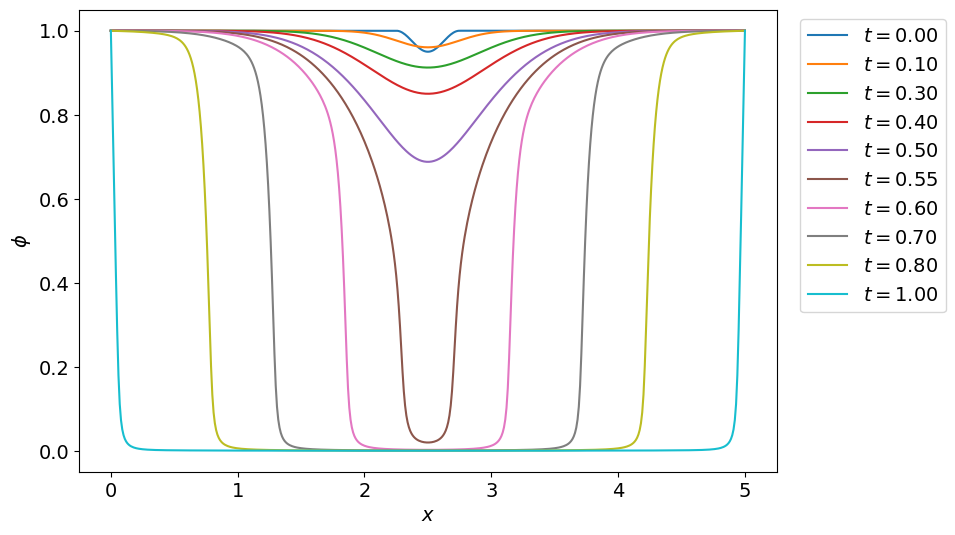
\includegraphics[width=\textwidth]{figures/typical_solution.png}
\end{figure}
\column{0.12\textwidth}
\hfill \\
\vspace{3.5cm}
\hspace{-2.5cm}
Узлов по измерениям: \\
\hspace{-2.5cm}
$N_x = 10^3$, $N_t = 10^5$
\end{columns}
\end{frame}


\begin{frame}{Вычисления: проверка устойчивости}
\vspace{-0.4cm}
\begin{columns}
\column{0.7\textwidth}
\begin{figure}
	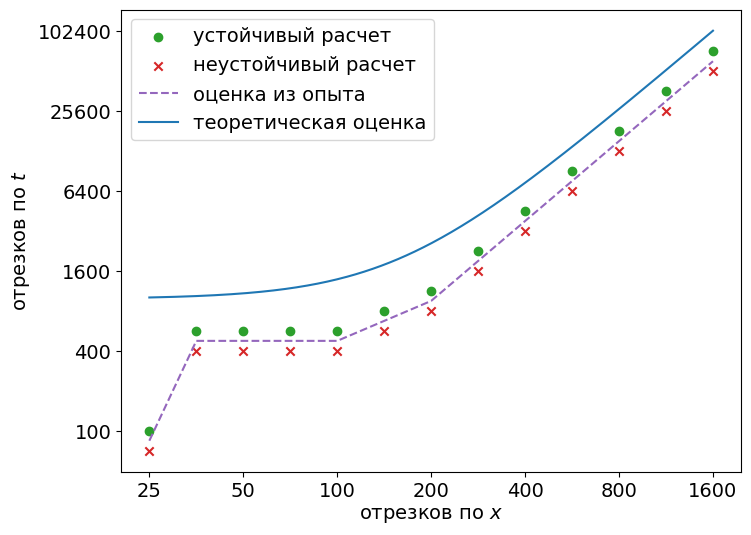
\includegraphics[width=\textwidth]{figures/stability_bounds.png}
\end{figure}
\column{0.3\textwidth}
Условие устойчивости:
$$\tau \leqslant \cfrac{1}{2m} \left( \cfrac{K_\Phi^2 \epsilon_0}{\delta^{5/3}} +
\cfrac{\Gamma}{h^2} \right)^{-1}$$
\end{columns}
\end{frame}


\begin{frame}{Вычисления: проверка сходимости}
\vspace{-0.3cm}
\begin{figure}
	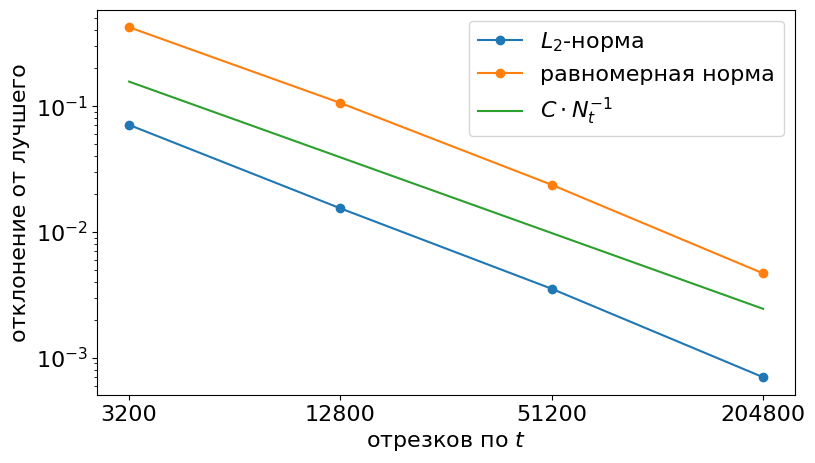
\includegraphics[width=0.58\textwidth]{figures/convergence_connected.png}
\end{figure}
\vspace{-0.6cm}
\begin{center}
	Здесь, согласно оценке устойчивости, $\tau = \cfrac{h^2}{4m \Gamma}$
\end{center}
\end{frame}


\begin{frame}{Вычисления: положения равновесия}
\vspace{-0.4cm}
\begin{center}
	$(1 + \delta)^2 < \cfrac{K_\Phi^2 l^2 \epsilon_0}{2 \Gamma}$ -- <<сильное>> напряжение
\end{center}
\vspace{-0.4cm}
\begin{columns}
\column{0.5\textwidth}
\begin{figure}
	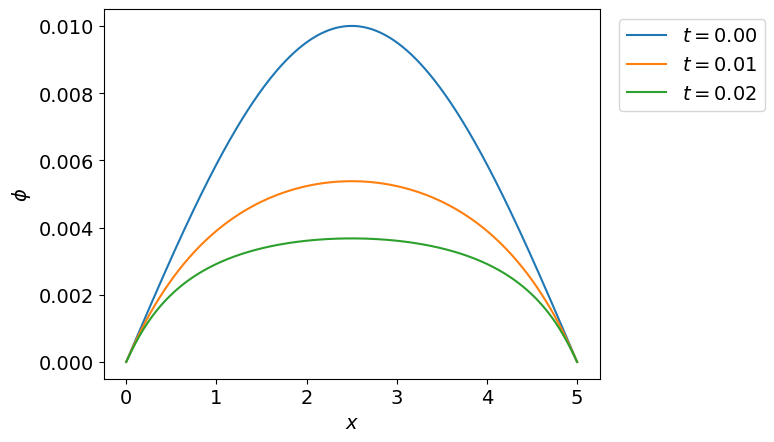
\includegraphics[width=\textwidth]{figures/equilibrium_3_0.png}
\end{figure}
\vspace{-0.8cm}
\begin{center}
	$\phi \equiv 0$, устойчивое
\end{center}
\column{0.5\textwidth}
\begin{figure}
	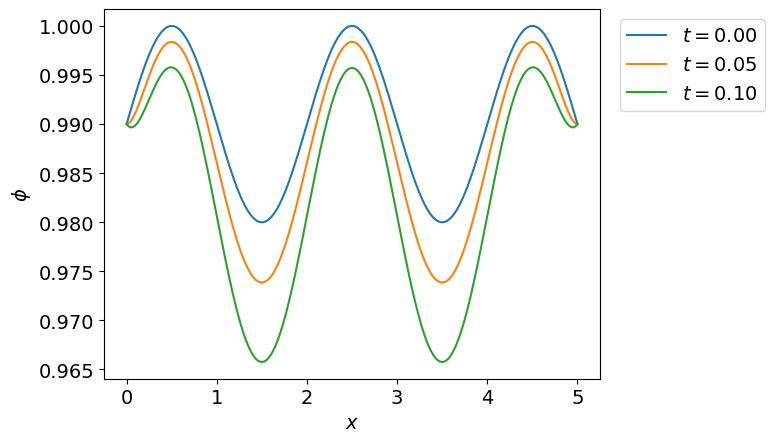
\includegraphics[width=\textwidth]{figures/equilibrium_3_1.png}
\end{figure}
\vspace{-0.8cm}
\begin{center}
	$\phi \equiv 1$, неустойчивое
\end{center}
\end{columns}
\end{frame}


\begin{frame}{Свободная энергия}
\vspace{-0.5cm}
$$\Pi(t) = \int\limits_\Omega \pi(x, t) dx$$
$$\pi = -\half \epsilon[\phi] \gradscalsq{\Phi} + \Gamma \left( \cfrac{1 - f(\phi)}{l^2} + \cfrac{1}{4} \gradscalsq{\phi} \right)$$
\begin{itemize}
	\item Уравнения \eqref{equation_potential}, \eqref{equation_phase} выведены так, что система в ходе эволюции стремится в состояние с как можно меньшей полной свободной энергией $\Pi$.
	\item Необходимо, чтобы указанное свойство выполнялось при моделировании.
\end{itemize}
\end{frame}


\begin{frame}{Вычисления: свободная энергия}
\vspace{-0.6cm}
\begin{figure}
	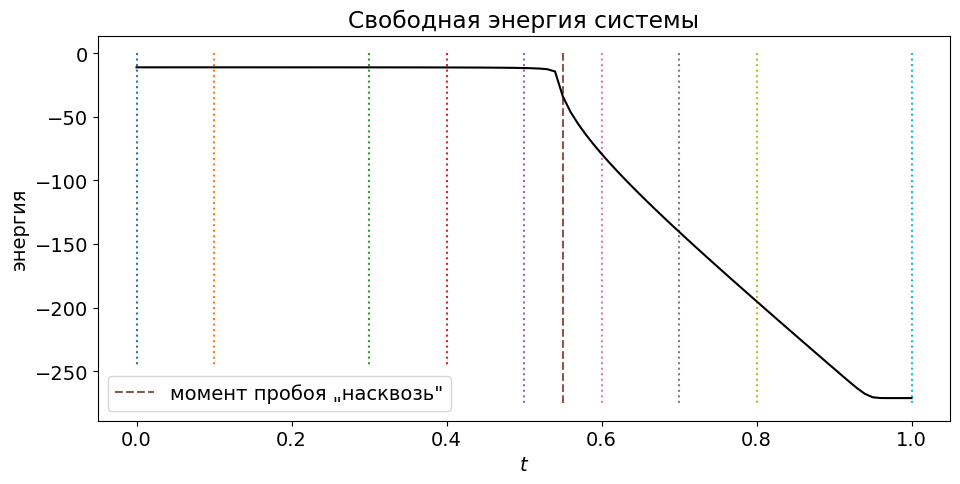
\includegraphics[width=0.88\textwidth]{figures/energy_total.png}
\end{figure}
\end{frame}

%!TEX root = ../main.tex

\section{Исследование обобщения модели}

\begin{frame}{Постановка задачи}
Исследуем распределение фазового поля вокруг проводников ($\phi = 0$) различного вида. Пусть $\Phi \equiv 0$. Рассмотрим следующие краевые задачи:
\begin{enumerate}
	\item $\Omega = [0, +\infty)_x \times I_y \times J_z$, $\phi|_{x = 0} = 0$, $\phi \to 1$ при $r = x \to +\infty$ -- плоский случай;
	\item $\Omega = \mathbb{R}_x \times \mathbb{R}_y \times J_z$, $\phi|_{x, y = 0} = 0$, $\phi \to 1$ при $r = \sqrt{x^2 + y^2} \to +\infty$ -- \\ цилиндрический случай;
	\item $\Omega = \mathbb{R}_x \times \mathbb{R}_y \times \mathbb{R}_z$, $\phi|_{x, y, z = 0} = 0$, $\phi \to 1$ при $r = \sqrt{x^2 + y^2 + z^2} \to +\infty$ -- \\
	сферический случай.
\end{enumerate}
Ищем стационарное решение $\phi = \phi(r)$.
\end{frame}


\begin{frame}{Суть проблемы}
\begin{columns}
\column{0.5\textwidth}
\centering
Плоский случай
\column{0.5\textwidth}
\centering
Цилиндрический случай
\end{columns}
\vspace{0.5cm}
\begin{columns}
\column{0.49\textwidth}
Задача Коши:
\vspace{-0.3cm}
$$\phi(0) = 0; \qquad \partx{\phi} = \cfrac{2}{l} \sqrt{1 - f(\phi)}$$
\begin{figure}
	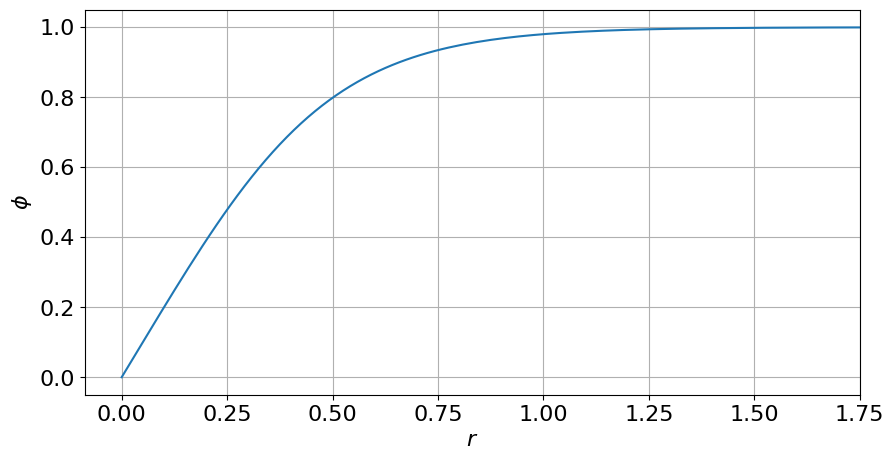
\includegraphics[width=\textwidth]{figures/result_volumes.png}
\end{figure}
\column{0.01\textwidth}
\rule{0.4pt}{0.7\textheight}
\column{0.49\textwidth}
\centering
Задача поставлена некорректно \\ и решения не имеет \cite{zipunova_higher_codimension}
\end{columns}
\end{frame}


\begin{frame}{Обобщение модели}
\vspace{-0.3cm}
\begin{block}{Обобщение модели, предложенное в работе \cite{zipunova_higher_codimension}}
\begin{itemize}
	\item Уравнение электрического потенциала $\Phi$:
	$$\Div(\epsilon[\phi] \nabla \Phi) = 0$$
	\item Уравнение фазового поля $\phi$:
	$$\cfrac{1}{m} \partt{\phi} = \half \epsilon'(\phi) \gradscalsq{\Phi} + \cfrac{\Gamma}{l^2} f'(\phi) + \half \Gamma \Delta \phi - \alpha \cfrac{\Gamma l^2}{4} \bilapl{\phi} + \beta \Gamma l^{p - 2} \plapl{\phi}{p - 2}$$
\end{itemize}
\end{block}
\begin{itemize}
	\item $\bilapl{\phi} = \Delta(\Delta \phi)$ -- билапласиан
	\item $\plapl{\phi}{p - 2}$ -- $p$-лапласиан
\end{itemize}
Везде далее $p = 4$.
\end{frame}


\begin{frame}{Разностная схема}
На границе $r = 0$ области моделирования у решения $\phi$ ожидается особенность. \\
Идея подхода:
\begin{itemize}
	\item используем метод конечных объемов: к ячейке $\Omega_i$ отнесено среднее
	$\widetilde{\phi}_i$ функции $\phi$;
	\item в первой и второй ячейках приближаем $\phi$ ЛК базисных функций, одна из которых имеет
	тот же вид особенности, что решение $\phi$;
	\item как и в классическом МКО, уравнения на $\widetilde{\phi}_i$ являются следствием
	балансовых соотношений.
\end{itemize}
Преимущества подхода:
\begin{itemize}
	\item точно учитываются граничные условия;
	\item точно учитывается асимптотика решения $\phi$ при $r \to 0$.
\end{itemize}
\end{frame}


\begin{frame}{Разностная схема}
$$\cfrac{1}{m} (\widetilde{\phi}_i^{j + 1} - \widetilde{\phi}_i^j) = \tau \cfrac{\Gamma}{l^2}
f'(\widetilde{\phi}_i^j) + \cfrac{\tau}{dV_i} \Gamma (\rho_{i + 1/2}^j S_{i + 1/2} -
\rho_{i - 1/2}^j S_{i - 1/2}) \text{;}$$
$$dV_i = r_{i + 1/2}^{k + 1} - r_{i - 1/2}^{k + 1}; \qquad
S_{i \pm 1/2} = (k + 1) r_{i \pm 1/2}^k \text{;}$$
$$\rho_{i \pm 1/2}^j = \half
\left[ \cfrac{\partial \phi}{\partial r} \right]_{i \pm 1/2}^j -
\alpha \cfrac{l^2}{4} \left[ \cfrac{\partial (\Delta \phi)}{\partial r} \right]_{i \pm 1/2}^j +
\beta l^2 \left( \left[ \cfrac{\partial \phi}{\partial r} \right]_{i \pm 1/2}^j \right)^3
\text{;}$$
$$\widetilde{\Delta \phi}_i^j = \cfrac{1}{dV_i}
\left( \left[ \cfrac{\partial \phi}{\partial r} \right]_{i + 1/2}^j S_{i + 1/2} -
\left[ \cfrac{\partial \phi}{\partial r} \right]_{i - 1/2}^j S_{i - 1/2} \right)$$
Подробнее в работе \cite{ponomarev_finite_volumes}.
\end{frame}


\begin{frame}{Полученные результаты}
\vspace{-1cm}
\begin{center}
	Предполагаемые виды особенности решения $\phi$ в точке $r = 0$
\end{center}
\begin{tabular}{|m{3cm}||m{3.5cm}|m{3.5cm}|m{3.5cm}|}
	\hline
	\vspace*{2mm} \hfill \vspace*{2mm} &\centering $\alpha = 0$, $\beta = 0$ &
	\centering $\alpha = 0$, $\beta \neq 0$ & \centering \arraybackslash $\alpha \neq 0$ \\
	\hline
	\hline
	\vspace{2mm} Плоский \linebreak случай \vspace{2mm} &
	\textcolor{green}{Без особенности} & \textcolor{green}{Без особенности} & \textcolor{green}{Без особенности} \\
	\hline
	\vspace{2mm} Цилиндрический \linebreak случай \vspace{2mm} &
	\textcolor{red}{Не имеет решения} & $r^{2/3}$ & $r^2 \ln r$ \\
	\hline
	\vspace{2mm} Сферический \linebreak случай \vspace{2mm} &
	\textcolor{red}{Предположительно не имеет решения} & $r^{1/3}$ & \textcolor{red}{Предположительно не имеет решения} \\
	\hline
\end{tabular}
\end{frame}


\begin{frame}{Полученные результаты}
\vspace{-0.6cm}
\begin{figure}
	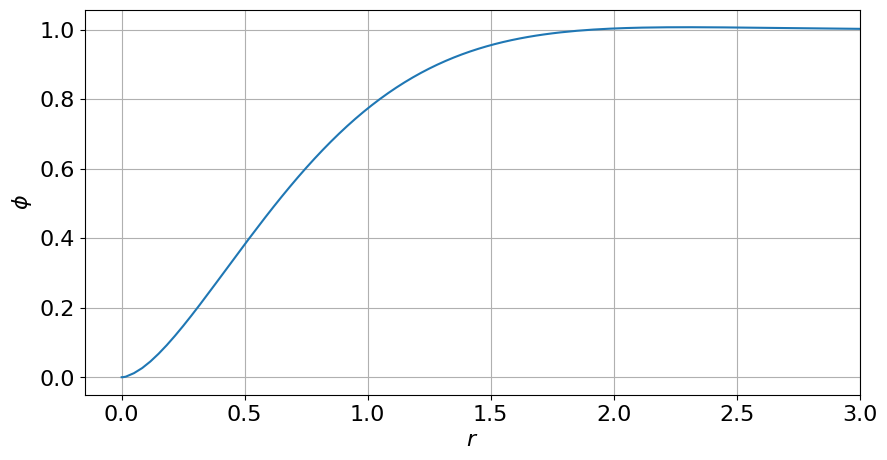
\includegraphics[width=0.81\textwidth]{figures/result_volumes_cyl_bi.png}
\end{figure}
\vspace{-0.7cm}
\begin{center}
	Цилиндрический случай, $\alpha = 1$: особенность вида $r^2 \ln r$
\end{center}
\end{frame}


\begin{frame}{Полученные результаты}
\vspace{-0.6cm}
\begin{figure}
	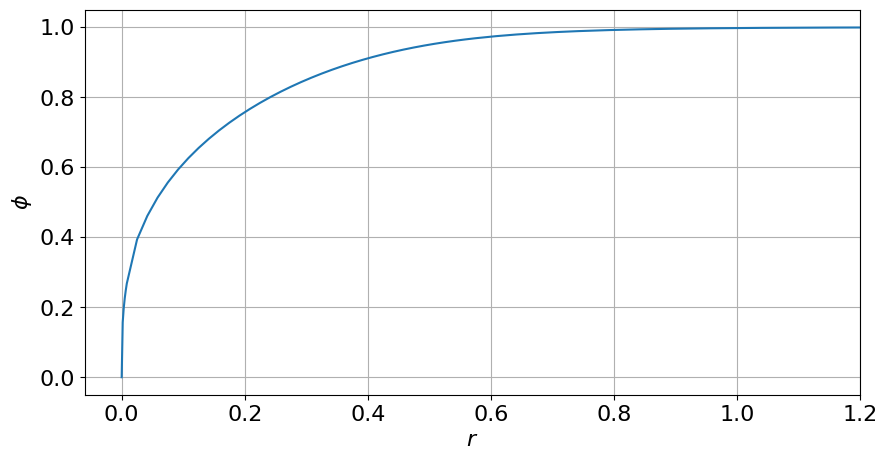
\includegraphics[width=0.81\textwidth]{figures/result_volumes_sph_p.png}
\end{figure}
\vspace{-0.7cm}
\begin{center}
	Сферический случай, $\alpha = 0$, $\beta = 1$: особенность вида $r^{1/3}$
\end{center}
\end{frame}

%!TEX root = ../main.tex

\section{Заключение}

Настоящая работа продолжает исследование, начатое в статье \cite{zipunova_higher_codimension}. Как было отмечено ее авторами, исследование это хотя и проводится для конкретной задачи, но, вероятно, затрагивает вопросы, содержащиеся в методе диффузной границы как таковом. Суть этих вопросов в том, позволяют ли уравнения среды с диффузной границей в своей <<классической>> редакции адекватно описывать включения, по своей природе являющиеся объектами высшей коразмерности. В качестве возможного ответа авторы работы \cite{zipunova_higher_codimension} предлагают определенного вида обобщение исходной модели.

Целью настоящей работы было численно исследовать упомянутое обобщение. В этом достигнуты определенные успехи. С помощью модификации метода конечных объемов преодолены трудности, связанные с необходимостью задавать граничные условия на множествах коразмерности 2 и 3 в трехмерном пространстве и с наличием у функции-решения  особенности в точках этих множеств. Указанный подход существенно не привязан к рассматриваемой модели -- в дальнейшем он может быть использован и в других задачах.

В некоторых случаях при построении разностной схемы возникали фундаментальные препятствия: оказывалось, что необходимых базисных функций попросту не существует. На основании этого выдвинута гипотеза, что в указанных случаях рассматриваемая дифференциальная задача поставлена некорректно и не имеет решения. Рассуждения вполне согласуется с теоретическими результатами работы \cite{zipunova_higher_codimension}. В будущем возможно строгое обоснование представленной гипотезы.


\begin{frame}{Литература}
\printbibliography
\end{frame}

\begin{frame}{}
\begin{center}
	\Large
	Спасибо за внимание!
\end{center}
\end{frame}

\end{document}